\documentclass[english, twocolumn, 10pt, aps, superscriptaddress, floatfix, prb, citeautoscript]{revtex4-1}
\pdfoutput=1
\usepackage[utf8]{inputenc}
\usepackage[T1]{fontenc}
\usepackage{listings}
\usepackage{units}
\usepackage{mathtools}
\usepackage{amsmath}
\usepackage{amssymb}
\usepackage{graphicx}
\usepackage{wasysym}
\usepackage{layouts}
\usepackage{siunitx}
\usepackage{bm}
\usepackage{xcolor}
\usepackage[colorlinks, citecolor={blue!50!black}, urlcolor={blue!50!black}, linkcolor={red!50!black}]{hyperref}
\usepackage{bookmark}
\usepackage{tabularx}
\usepackage{microtype}
\usepackage{babel}
\usepackage{textcomp}
\hypersetup{pdfauthor={Tinkerer},pdftitle={\emph{Adaptive}: an adaptive parallel sampling algorithm for mathematical functions based on local local criteria}}

\setcounter{secnumdepth}{4}
\setcounter{tocdepth}{4}

\newcounter{CommentNumber}
% \renewcommand{\paragraph}[1]{\stepcounter{CommentNumber}\belowpdfbookmark{#1}{\arabic{CommentNumber}}}

\DeclarePairedDelimiter\abs{\lvert}{\rvert}
\DeclarePairedDelimiter\norm{\lVert}{\rVert}

\makeatletter
\let\oldabs\abs
\def\abs{\@ifstar{\oldabs}{\oldabs*}}
\let\oldnorm\norm
\def\norm{\@ifstar{\oldnorm}{\oldnorm*}}
\makeatother

\newcommand{\ev}[1]{\langle#1\rangle}
\newcommand{\bra}[1]{\langle#1|}
\newcommand{\ket}[1]{|#1\rangle}
\newcommand{\bracket}[2]{\langle#1|#2\rangle}

\newcolumntype{L}[1]{>{\raggedright\arraybackslash}p{#1}}
\newcolumntype{C}[1]{>{\centering\arraybackslash}p{#1}}
\newcolumntype{R}[1]{>{\raggedleft\arraybackslash}p{#1}}

% workaround for https://github.com/jgm/pandoc/issues/2392#issuecomment-140114736
\renewcommand{\citep}{\cite}

% workaround for https://github.com/jgm/pandoc/issues/4716
\newcommand{\passthrough}[1]{\lstset{mathescape=false}#1\lstset{mathescape=true}}

% listing settings, from https://tex.stackexchange.com/a/179956
\lstset{
    basicstyle=\ttfamily,
    numbers=left,
    keywordstyle=\color[rgb]{0.13,0.29,0.53}\bfseries,
    stringstyle=\color[rgb]{0.31,0.60,0.02},
    commentstyle=\color[rgb]{0.56,0.35,0.01}\itshape,
    numberstyle=\footnotesize,
    stepnumber=1,
    numbersep=5pt,
    backgroundcolor=\color[RGB]{248,248,248},
    showspaces=false,
    showstringspaces=false,
    showtabs=false,
    tabsize=2,
    captionpos=b,
    breaklines=true,
    breakatwhitespace=true,
    breakautoindent=true,
    escapeinside={\%*}{*)},
    linewidth=\columnwidth,
    basewidth=0.5em,
}


\begin{document}

\title{\emph{Adaptive}: an adaptive parallel sampling algorithm for mathematical functions based on local local criteria}

\author{Tinkerer}
\email[Electronic address: ]{bas@nijho.lt}
\affiliation{Kavli Institute of Nanoscience, Delft University of Technology, P.O. Box 4056, 2600 GA Delft, The Netherlands}

\date{\today}

\begin{abstract}
Large scale computer simulations are time-consuming to run and often require sweeps over input parameters to obtain a qualitative understanding of the simulation output.
These sweeps of parameters can potentially make the simulations prohibitively expensive.
Therefore, when evaluating a function numerically, it is advantageous to sample it more densely in the interesting regions (called adaptive sampling) instead of evaluating it on a manually-defined homogeneous grid.
Such adaptive algorithms exist within the machine learning field.
These methods can suggest a new point to calculate based on \emph{all} existing data at that time; however, this is an expensive operation.
An alternative is to use local algorithms---in contrast to the previously mentioned global algorithms---which can suggest a new point, based only on the data in the immediate vicinity of a new point.
This approach works well, even when using hundreds of computers simultaneously because the point suggestion algorithm is cheap (fast) to evaluate.
We provide a reference implementation in Python and show its performance.
\end{abstract}

\flushbottom
\maketitle

\section{Introduction}

\paragraph{Simulations are costly and often require sampling a region in parameter space.}

In the computational sciences, one often does costly simulations---represented by a function \(f\)---where a certain region in parameter space \(X\) is sampled, mapping to a codomain \(Y\): \(f \colon X \to Y\).
Frequently, the different points in \(X\) can be independently calculated.
Even though it is suboptimal, one usually resorts to sampling \(X\) on a homogeneous grid because of its simple implementation.

\paragraph{Choosing new points based on existing data improves the simulation efficiency.}

An alternative, which improves the simulation efficiency, is to choose new potentially interesting points in \(X\), based on existing data \citep{Gramacy2004, Figueiredo1995, Castro2008, Chen2017}.
Bayesian optimization works well for high-cost simulations where one needs to find a minimum (or maximum) \citep{Takhtaganov2018}.
However, if the goal of the simulation is to approximate a continuous function using the fewest points, an alternative strategy is to use a greedy algorithm that samples mid-points of intervals with the largest length or curvature \citep{Wolfram2011}.
Such a sampling strategy (i.e., in Fig.~\ref{fig:algo}) would trivially speedup many simulations.
Another advantage of such an algorithm is that it may be parallelized cheaply (i.e.~more than one point may be sampled at a time), as we do not need to perform a global computation over all the data (as we would with Bayesian sampling) when determining which points to sample next.

\begin{figure}
\centering
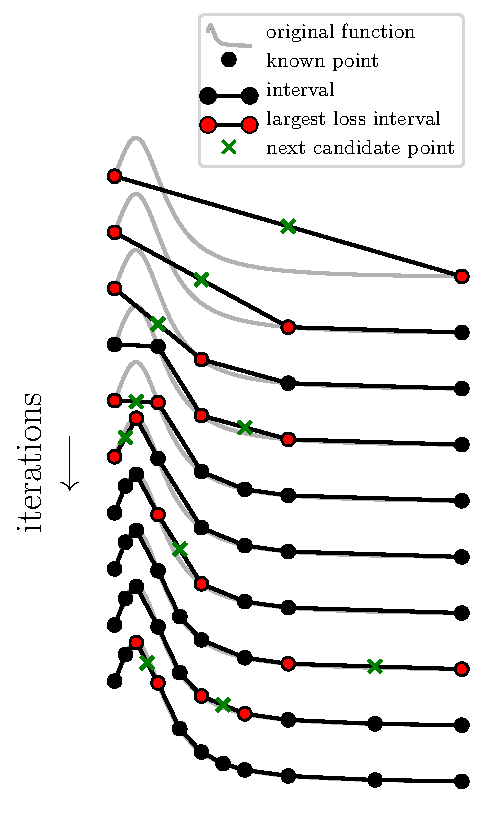
\includegraphics{figures/algo.pdf}
\caption{Visualization of a 1-D sampling strategy for a black-box function (grey).
We start by calculating the two boundary points.
Two adjacent existing data points (black) \(\{x_i, y_i\}\) define an interval.
Each interval has a loss \(L_{i,i+1}\) associated with it that can be calculated from the points inside the interval \(L_{i,i+1}(x_i, x_{i+1}, y_i, y_{i+1})\) and optionally of \(N\) next nearest neighboring intervals.
At each iteration the interval with the largest loss is indicated (red), with its corresponding candidate point (green) picked in the middle of the interval.
The loss function in this example is an approximation to the curvature, calculated using the data from an interval and its nearest neighbors.\label{fig:algo}}
\end{figure}

\paragraph{We describe a class of algorithms relying on local criteria for sampling, which allow for easy parallelization and have a low overhead.}

The algorithm visualized in \ref{fig:algo} consists of the following steps:
(1) evaluate the function at the boundaries \(a\) and \(b\), of the interval of interest,
(2) calculate the loss for the interval \(L_{a, b} = \sqrt{(b - a)^2 + (f(b) - f(a))^2}\),
(3) pick a new point \(x_\textrm{new}\) in the centre of the interval with the largest loss, \((x_i, x_j)\),
(4) calculate \(f(x_\textrm{new})\),
(5) discard the interval \((x_i, x_j)\) and create two new intervals \((x_i, x_\textrm{new})\) and \((x_\textrm{new}, x_j)\), calculating their losses \(L_{x_i, x_\textrm{new}}\) and \(L_{x_\textrm{new}, x_j}\)
(6) repeat from step 3.

In this paper we present a class of algorithms that generalizes the above example.
This general class of algorithms is based on using a \emph{priority queue} of subdomains (intervals in 1-D), ordered by a \emph{loss} obtained from a \emph{local loss function} (which depends only on the data local to the subdomain), and greedily selecting points from subdomains at the top of the priority queue.
The advantage of these \emph{local} algorithms is that they have a lower computational overhead than algorithms requiring \emph{global} data and updates (e.g.~Bayesian sampling), and are therefore more amenable to parallel evaluation of the function of interest.

\begin{figure}
\centering
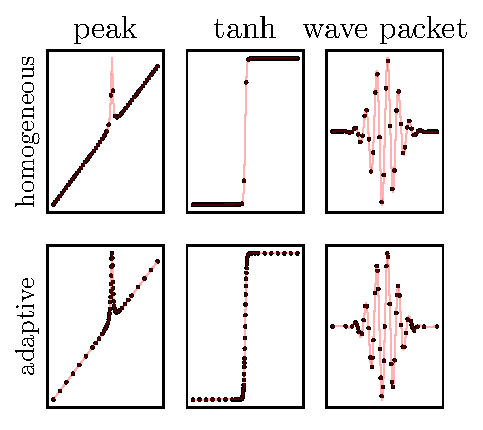
\includegraphics{figures/Learner1D.pdf}
\caption{Comparison of homogeneous sampling (top) with adaptive sampling (bottom) for different one-dimensional functions (red) where the number of points in each column is identical.
We see that when the function has a distinct feature---such as with the peak and tanh---adaptive sampling performs much better.
When the features are homogeneously spaced, such as with the wave packet, adaptive sampling is not as effective as in the other cases.\label{fig:Learner1D}}
\end{figure}

\begin{figure}
\centering
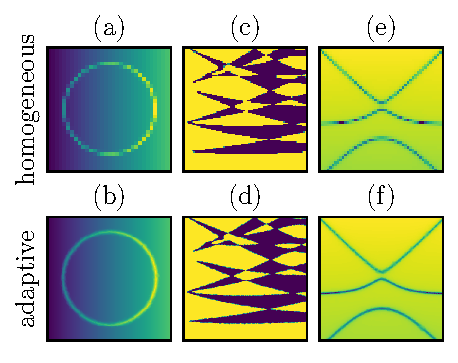
\includegraphics{figures/Learner2D.pdf}
\caption{Comparison of homogeneous sampling (top) with adaptive sampling (bottom) for different two-dimensional functions where the number of points in each column is identical.
On the left is the function \(f(x) = x + a ^ 2 / (a ^ 2 + (x - x_\textrm{offset}) ^ 2)\).
In the middle a topological phase diagram from \onlinecite{Nijholt2016}, where the function can take the values -1 or 1.
On the right, we plot level crossings for a two-level quantum system.
In all cases using Adaptive results in a higher fidelity plot.\label{fig:Learner2D}}
\end{figure}

\paragraph{We provide a reference implementation, the Adaptive package, and demonstrate its performance.}

We provide a reference implementation, the open-source Python package called Adaptive \citep{Nijholt2019}, which has previously been used in several scientific publications \citep{Vuik2018, Laeven2019, Bommer2019, Melo2019}.
It has algorithms for \(f \colon \mathbb{R}^N \to \mathbb{R}^M\), where \(N, M \in \mathbb{Z}^+\) but which work best when \(N\) is small; integration in \(\mathbb{R}\); and the averaging of stochastic functions.
Most of our algorithms allow for a customizable loss function with which one can adapt the sampling algorithm to work optimally for different classes of functions.
It integrates with the Jupyter notebook environment as well as popular parallel computation frameworks such as \passthrough{\lstinline!ipyparallel!}, \passthrough{\lstinline!mpi4py!}, and \passthrough{\lstinline!dask.distributed!}.
It provides auxiliary functionality such as live-plotting, inspecting the data as the calculation is in progress, and automatically saving and loading of the data.

The raw data and source code that produces all plots in this paper is available at \onlinecite{papercode}.

\hypertarget{sec:review}{%
\section{Review of adaptive sampling}\label{sec:review}}

Optimal sampling and planning based on data is a mature field with different communities providing their own context, restrictions, and algorithms to solve their problems.
To explain the relation of our approach with prior work, we discuss several existing contexts.
This is not a systematic review of all these fields, but rather, we aim to identify the important traits and design considerations.

\paragraph{Experiment design uses Bayesian sampling because the computational costs are not a limitation.}

Optimal experiment design (OED) is a field of statistics that minimizes the number of experimental runs needed to estimate specific parameters and, thereby, reduce the cost of experimentation \citep{Emery1998}.
It works with many degrees of freedom and can consider constraints, for example, when the sample space contains regions that are infeasible for practical reasons.
One form of OED is response-adaptive design \citep{Hu2006}, which concerns the adaptive sampling of designs for statistical experiments.
Here, the acquired data (i.e., the observations) are used to estimate the uncertainties of a certain desired parameter.
It then suggests further experiments that will optimally reduce these uncertainties.
In this step of the calculation Bayesian statistics is frequently used.
Bayesian statistics naturally provides tools for answering such questions; however, because it provides closed-form solutions, Markov chain Monte Carlo (MCMC) sampling is the standard tool for determining the most promising samples.
In a typical non-adaptive experiment, decisions on which experiments to perform are made in advance.

\paragraph{Plotting and low dimensional integration uses local sampling.}

Plotting a low dimensional function in between bounds requires one to evaluate the function on sufficiently many points such that when we interpolate values in between data points, we get an accurate description of the function values that were not explicitly calculated.
In order to minimize the number of function evaluations, one can use adaptive sampling routines.
For example, for one-dimensional functions, Mathematica \citep{WolframResearch} implements a \passthrough{\lstinline!FunctionInterpolation!} class that takes the function, \(x_\textrm{min}\), and \(x_\textrm{max}\), and returns an object that samples the function more densely in regions with high curvature; however, details on the algorithm are not published.
Subsequently, we can query this object for points in between \(x_\textrm{min}\) and \(x_\textrm{max}\), and get the interpolated value, or we can use it to plot the function without specifying a grid.
Another application for adaptive sampling is numerical integration.
It works by estimating the integration error of each interval and then minimizing the sum of these errors greedily.
For example, the \passthrough{\lstinline!CQUAD!} algorithm \citep{Gonnet2010} in the GNU Scientific Library \citep{Galassi1996} implements a more sophisticated strategy and is a doubly-adaptive general-purpose integration routine which can handle most types of singularities.
In general, it requires more function evaluations than the integration routines in \passthrough{\lstinline!QUADPACK!} \citep{Galassi1996}; however, it works more often for difficult integrands.
It is doubly-adaptive because it can decide to either subdivide intervals into more intervals or refine an interval by using a polynomial approximation of higher degree, requiring more points.

\paragraph{PDE solvers and computer graphics use adaptive meshing.}

Hydrodynamics \citep{Berger1989, Berger1984} and astrophysics \citep{Klein1999} use an adaptive refinement of the triangulation mesh on which a partial differential equation is discretized.
By providing smaller mesh elements in regions with a higher variation of the solution, they reduce the amount of data and calculation needed at each step of time propagation.
The remeshing at each time step happens globally, and this is an expensive operation.
Therefore, mesh optimization does not fit our workflow because expensive global updates should be avoided.
Computer graphics uses similar adaptive methods where a smooth surface can represent a surface via a coarser piecewise linear polygon mesh, called a subdivision surface \citep{DeRose1998}.
An example of such a polygonal remeshing method is one where the polygons align with the curvature of the space or field; this is called anisotropic meshing \citep{Alliez2003}.

\hypertarget{sec:design}{%
\section{Design constraints and the general algorithm}\label{sec:design}}

\paragraph{We aim to sample low to intermediate cost functions in parallel.}

The general algorithm that we describe in this paper works best for low to intermediate cost functions.
Determining the next candidate points happens in a single sequential process while the function executions can be in parallel.
This means that to benefit from an adaptive sampling algorithm, that the time it takes to suggest a new point \(t_\textrm{suggest}\) must be much smaller than the average function execution time \(t_f\) over the number of parallel workers \(N\): \(t_f / N \gg t_\textrm{suggest}\).
Functions that are fast to evaluate can be calculated on a dense grid, and functions that are slow to evaluate might benefit from full-scale Bayesian optimization where \(t_\textrm{suggest}\) is large.
We are interested in the intermediate case, when one wishes to sample adaptively, but cannot afford the luxury of fitting of all available data at each step.
While this may seem restrictive, we assert that a large class of functions is inside the right regime for local adaptive sampling to be beneficial.

\paragraph{We propose to use a local loss function as a criterion for choosing the next point.}

Because we aim to keep the suggestion time \(t_\textrm{suggest}\) small, we propose to use the following approach, which operates on a constant-size subset of the data to determine which point to suggest next.
We keep track of the subdomains in a priority queue, where each subdomain is assigned a priority called the ``loss''.
To suggest a new point we remove the subdomain with the largest loss from the priority queue and select a new point \(x_\textrm{new}\) from within it (typically in the centre)
This splits the subdomain into several smaller subdomains \(\{S_i\}\) that each contain \(x_\textrm{new}\) on their boundaries.
After evaluating the function at \(x_\textrm{new}\) we must then recompute the losses using the new data.
We choose to consider loss functions that are ``local'', i.e.~the loss for a subdomain depends only on the points contained in that subdomain and possibly a (small) finite number of neighboring subdomains.
This means that we need only recalculate the losses for subdomains that are ``close'' to \(x_\textrm{new}\).
Having computed the new losses we must then insert the \(\{S_i\}\) into the priority queue, and also update the priorities of the neighboring subdomains, if their loss was recalculated.
After these insertions and updates we are ready to suggest the next point to evaluate.
Due to the local nature of this algorithm and the sparsity of space in higher dimensions, we will suffer from the curse of dimensionality.
The algorithm, therefore, works best in low dimensional space; typically calculations that can reasonably be plotted, so with 1, 2, or 3 degrees of freedom.

\paragraph{We summarize the algorithm with pseudocode}

The algorithm described above can be made more precise by the following Python code:

\begin{lstlisting}[language=Python]
first_subdomain, = domain.subdomains()
for x in domain.points(first_subdomain):
  data[x] = f(x)

queue.insert(first_subdomain, priority=loss(domain, first_subdomain, data))

while queue.max_priority() < target_loss:
  loss, subdomain = queue.pop()

  new_points, new_subdomains = domain.split(subdomain)
  for x in new_points:
    data[x] = f(x)

  for subdomain in new_subdomains:
    queue.insert(subdomain, priority=loss(domain, subdomain, data))

  if loss.n_neighbors > 0:
    subdomains_to_update = set()
    for d in new_subdomains:
      neighbors = domain.neighbors(d, loss.n_neighbors)
      subdomains_to_update.update(neighbors)
    subdomains_to_update -= set(new_subdomains)
    for subdomain in subdomains_to_update:
      queue.update(subdomain, priority=loss(domain, subdomain, data))
\end{lstlisting}

where we have used the following definitions:

\begin{description}
\item[\texttt{f}]
The function we wish to learn
\item[\texttt{queue}]
A priority queue of unique elements, supporting the following methods: \passthrough{\lstinline!max\_priority()!}, to get the priority of the top element; \passthrough{\lstinline!pop()!}, remove and return the top element and its priority; \passthrough{\lstinline!insert(element, priority)!}, insert the given element with the given priority into the queue;\passthrough{\lstinline!update(element, priority)!}, update the priority of the given element, which is already in the queue.
\item[\texttt{domain}]
An object representing the domain of \passthrough{\lstinline!f!} split into subdomains. Supports the following methods: \passthrough{\lstinline!subdomains()!}, returns all the subdomains; \passthrough{\lstinline!points(subdomain)!}, returns all the points contained in the provided subdomain; \passthrough{\lstinline!split(subdomain)!}, splits a subdomain into smaller subdomains, returning the new points and new subdomains produced as a result; \passthrough{\lstinline!neighbors(subdomain, n\_neighbors)!}, returns the subdomains neighboring the provided subdomain.
\item[\texttt{data}]
A hashmap storing the points \passthrough{\lstinline!x!} and their values \passthrough{\lstinline!f(x)!}.
\item[\texttt{loss(domain,\ subdomain,\ data)}]
The loss function, with \passthrough{\lstinline!loss.n\_neighbors!} being the degree of neighboring subdomains that the loss function uses.
\end{description}

\paragraph{As an example, the interpoint distance is a good loss function in one dimension.}

An example of such a local loss function for a one-dimensional function is the interpoint distance, i.e.~given a subdomain (interval) \((x_\textrm{a}, x_\textrm{b})\) with values \((y_\textrm{a}, y_\textrm{b})\) the loss is \(\sqrt{(x_\textrm{a} - x_\textrm{b})^2 + (y_\textrm{a} - y_\textrm{b})^2}\).
A more complex loss function that also takes the first neighboring intervals into account is one that approximates the second derivative using a Taylor expansion.
Figure \ref{fig:Learner1D} shows a comparison between a result using this loss and a function that is sampled on a grid.

\paragraph{This algorithm has a logarithmic overhead when combined with an appropriate data structure}

The key data structures in the above algorithm are \passthrough{\lstinline!queue!} and \passthrough{\lstinline!domain!}.
The priority queue must support efficiently finding and removing the maximum priority element, as well as updating the priority of arbitrary elements whose priority is unknown (when updating the loss of neighboring subdomains).
Such a datastructure can be achieved with a combination of a hashmap (mapping elements to their priority) and a red--black tree or a skip list \citep{Cormen2009} that stores \passthrough{\lstinline!(priority, element)!}.
This has average complexity of \(\mathcal{O}(\log{n})\) for all the required operations.
In the reference implementation, we use the SortedContainers Python package \citep{Jenks2014}, which provides an efficient implementation of such a data structure optimized for realistic sizes, rather than asymptotic complexity.
The \passthrough{\lstinline!domain!} object requires efficiently splitting a subdomain and querying the neighbors of a subdomain.
For the one-dimensional case this can be achieved by using a red--black tree to keep the points \(x\) in ascending order.
In this case both operations have an average complexity of \(\mathcal{O}(\log{n})\).
In the reference implementation we again use SortedContainers.
We thus see that by using the appropriate data structures the time required to suggest a new point is \(t_\textrm{suggest} \propto \mathcal{O}(\log{n})\).
The total time spent on suggesting points when sampling \(N\) points in total is thus \(\mathcal{O}(N \log{N})\).

\paragraph{With many points, due to the loss being local, parallel sampling incurs no additional cost.}

So far, the description of the general algorithm did not include parallelism.
In order to include parallelism we need to allow for points that are ``pending'', i.e.~whose value has been requested but is not yet known.
In the sequential algorithm subdomains only contain points on their boundaries.
In the parallel algorithm \emph{pending} points are placed in the interior of subdomains, and the priority of the subdomains in the queue is reduced to take these pending points into account.
Later, when a pending point \(x\) is finally evaluated, we \emph{split} the subdomain that contains \(x\) such that it is on the boundary of new, smaller, subdomains.
We then calculate the priority of these new subdomains, and insert them into the priority queue, and update the priority of neighboring subdomains if required.

\paragraph{We summarize the algorithm with pseudocode}

The parallel version of the algorithm can be described by the following Python code:

\begin{lstlisting}[language=Python]
def priority(domain, subdomain, data):
    subvolumes = domain.subvolumes(subdomain)
    max_relative_subvolume = max(subvolumes) / sum(subvolumes)
    L_0 = loss(domain, subdomain, data)
    return max_relative_subvolume * L_0

first_subdomain, = domain.subdomains()
for x in domain.points(first_subdomain):
  data[x] = f(x)

new_points = domain.insert_points(first_subdomain, executor.ncores)
for x in new_points:
  data[x] = None
  executor.submit(f, x)

queue.insert(first_subdomain, priority=priority(domain, subdomain, data))

while executor.n_outstanding_points > 0:
  x, y = executor.get_one_result()
  data[x] = y

  # Split into smaller subdomains with `x` at a subdomain boundary
  # And calculate the losses for these new subdomains
  old_subdomains, new_subdomains = domain.split_at(x)
  for subdomain in old_subdomains:
    queue.remove(old_subdomain)
  for subdomain in new_subdomains:
    queue.insert(subdomain, priority(domain, subdomain, data))

  if loss.n_neighbors > 0:
    subdomains_to_update = set()
    for d in new_subdomains:
      neighbors = domain.neighbors(d, loss.n_neighbors)
      subdomains_to_update.update(neighbors)
    subdomains_to_update -= set(new_subdomains)
    for subdomain in subdomains_to_update:
      queue.update(subdomain, priority(domain, subdomain, data))

  # If it looks like we're done, don't send more work
  if queue.max_priority() < target_loss:
    continue

  # Send as many points for evaluation as we have compute cores
  for _ in range(executor.ncores - executor.n_outstanding_points)
    loss, subdomain = queue.pop()
    new_point, = domain.insert_points(subdomain, 1)
    data[new_point] = None
    executor.submit(f, new_point)
    queue.insert(subdomain, priority(domain, subdomain, data))
\end{lstlisting}

Where we have used identical definitions to the serial case for \passthrough{\lstinline!f!}, \passthrough{\lstinline!data!}, \passthrough{\lstinline!loss!} and the following additional definitions:

\begin{description}
\item[\texttt{queue}]
As for the sequential case, but must additionally support: \passthrough{\lstinline!remove(element)!}, remove the provided element from the queue.
\item[\texttt{domain}]
As for the sequential case, but must additionally support: \passthrough{\lstinline!insert\_points(subdomain, n)!}, insert \passthrough{\lstinline!n!} (pending) points into the given subdomain without splitting the subdomain; \passthrough{\lstinline!subvolumes(subdomain)!}, return the volumes of all the sub-subdomains contained within the given subdomain; \passthrough{\lstinline!split\_at(x)!}, split the domain at a new (evaluated) point \passthrough{\lstinline!x!}, returning the old subdomains that were removed, and the new subdomains that were added as a result.
\item[\texttt{executor}]
An object that can submit function evaluations to computing resources and retrieve results.
Supports the following methods: \passthrough{\lstinline!submit(f, x)!}, schedule the execution of \passthrough{\lstinline!f(x)!} and do not block ; \passthrough{\lstinline!get\_one\_result()!}, block waiting for a single result, returning the pair \passthrough{\lstinline!(x, y)!} as soon as it becomes available; \passthrough{\lstinline!ncores!}, the total number of parallel processing units; \passthrough{\lstinline!n\_outstanding\_points!}, the number of function evaluations that have been requested and not yet retrieved, incremented by \passthrough{\lstinline!submit!} and decremented by \passthrough{\lstinline!get\_one\_result!}.
\end{description}

\hypertarget{sec:loss}{%
\section{Loss function design}\label{sec:loss}}

\paragraph{Sampling in different problems pursues different goals}

Not all goals are achieved by using an identical sampling strategy; the specific problem determines the goal.
For example, quadrature rules requires a denser sampling of the subdomains where the interpolation error is highest, plotting (or function approximation) requires continuity of the approximation, maximization only cares about finding an optimum, and isoline or isosurface sampling aims to sample regions near a given function value more densely.
These different sampling goals each require a loss function tailored to the specific case.

\paragraph{Different loss functions tailor sampling performance for different classes of functions}

Additionally, it is important to take the class of functions being learned when selecting a loss function into account, even if the specific goal (e.g.~continuity of the approximation) remains unchanged.
For example, if we wanted a smooth approximation to a function with a singularity, then the interpoint distance loss function would be a poor choice, even if it is generally a good choice for that specified goal.
This is because the aforementioned loss function will ``lock on'' to the singularity, and will fail to sample the function elsewhere once it starts.
This is an illustration of the following principle: for optimal sampling performance, loss functions should be tailored to the particular domain of interest.

\paragraph{Loss function regularization avoids singularities}

One strategy for designing loss functions is to take existing loss functions and apply a regularization.
For example, to limit the over-sampling of singularities inherent in the distance loss we can set the loss of subdomains that are smaller than a given threshold to zero, which will prevent them from being sampled further.

\paragraph{Adding loss functions allows for balancing between multiple priorities.}

Another general strategy for designing loss functions is to combine existing loss functions that optimize for particular features, and then combine them together.
Typically one weights the different constituent losses to prioritize the different features.
For example, combining a loss function that calculates the curvature with a distance loss function will sample regions with high curvature more densely, while ensuring continuity.
Another important example is combining a loss function with the volume of the subdomain, which will ensure that the sampling is asymptotically dense everywhere (because large subdomains will have a correspondingly large loss).
This is important if there are many distinct and narrow features that all need to be found, and densely sampled in the region around the feature.

\section{Examples}

\subsection{Line simplification loss}

\paragraph{The line simplification loss is based on an inverse Visvalingam's algorithm.}

Inspired by a method commonly employed in digital cartography for coastline simplification, Visvalingam's algorithm, we construct a loss function that does its reverse \citep{Visvalingam1990}.
Here, at each point (ignoring the boundary points), we compute the effective area associated with its triangle, see Fig.~\ref{fig:line_loss}(b).
The loss then becomes the average area of two adjacent triangles.
By Taylor expanding \(f\) around \(x\) it can be shown that the area of the triangles relates to the contributions of the second derivative.
We can generalize this loss to \(N\) dimensions, where the triangle is replaced by a \((N+1)\) dimensional simplex.

\begin{figure}
\centering
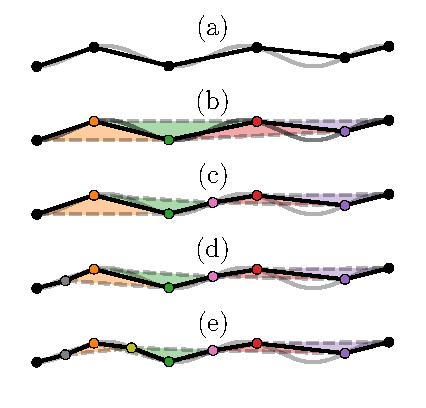
\includegraphics{figures/line_loss.pdf}
\caption{Line loss visualization.
In this example, we start with 6 points (a) on the function (grey).
Ignoring the endpoints, the effective area of each point is determined by its associated triangle (b).
The loss of each interval can be computed by taking the average area of the adjacent triangles.
Subplots (c), (d), and (e) show the subsequent iterations following (b).\label{fig:line_loss}}
\end{figure}

In order to compare sampling strategies, we need to define some error.
We construct a linear interpolation function \(\tilde{f}\), which is an approximation of \(f\).
We calculate the error in the \(L^{1}\)-norm, defined as,
\[
\text{Err}_{1}(\tilde{f})=\left\Vert \tilde{f}-f\right\Vert _{L^{1}}=\int_{a}^{b}\left|\tilde{f}(x)-f(x)\right|\text{d}x.
\]
This error approaches zero as the approximation becomes better.

\begin{figure}
\centering
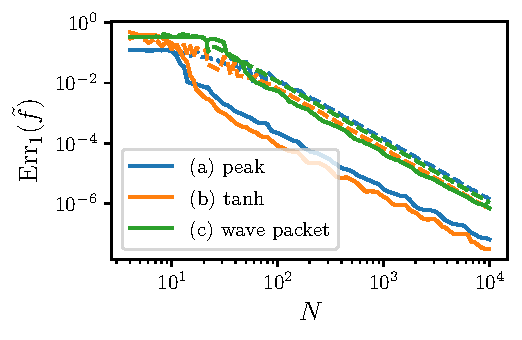
\includegraphics{figures/line_loss_error.pdf}
\caption{The \(L^{1}\)-norm error as a function of number of points \(N\) for the functions in Fig.~\ref{fig:Learner1D} (a,b,c).
The interrupted lines correspond to homogeneous sampling and the solid line to the sampling with the line loss.
In all cases adaptive sampling performs better, where the error is a factor 1.6-20 lower for \(N=10000\).\label{fig:line_loss_error}}
\end{figure}

Figure \ref{fig:line_loss_error} shows this error as a function of the number of points \(N\).
Here, we see that for homogeneous sampling to get the same error as sampling with a line loss, a factor \(\approx 1.6-20\) times more points are needed, depending on the function.

\subsection{A parallelizable adaptive integration algorithm based on cquad}

\paragraph{\texorpdfstring{The \texttt{cquad} algorithm belongs to a class that is parallelizable.}{The cquad algorithm belongs to a class that is parallelizable.}}

In Sec.~\ref{sec:review} we mentioned the doubly-adaptive integration algorithm \passthrough{\lstinline!CQUAD!} \citep{Gonnet2010}.
This algorithm uses a Clenshaw-Curtis quadrature rules of increasing degree \(d\) in each interval \citep{Clenshaw1960}.
The error estimate is \(\sqrt{\int{\left(f_0(x) - f_1(x)\right)^2}}\), where \(f_0\) and \(f_1\) are two successive interpolations of the integrand.
To reach the desired total error, intervals with the maximum absolute error are improved.
Either (1) the degree of the rule is increased or (2) the interval is split if either the function does not appear to be smooth or a rule of maximum degree (\(d=4\)) has been reached.
All points inside the intervals can be trivially calculated in parallel; however, when there are more resources available than points, Adaptive needs to guess whether an (1) interval's should degree of the rule should be increased or (2) or the interval is split.
Here, we choose to always increase until \(d=4\), after which the interval is split.

\subsection{isoline and isosurface sampling}

A judicious choice of loss function allows to sample the function close to an isoline (isosurface in 2D). Specifically, we prioritize subdomains that are bisected by the isoline or isosurface:

\begin{lstlisting}[language=Python]
def isoline_loss_function(level, priority):
    def loss(simplex, values, value_scale):
        values = np.array(values)
        which_side = np.sign(level * value_scale - values)
        crosses_isoline = np.any(np.diff(which_side))
        return volume(simplex)* (1 + priority * crosses_isoline)
    return loss
\end{lstlisting}

See Fig.~\ref{fig:isoline} for a comparison with uniform sampling.

\begin{figure}
\centering
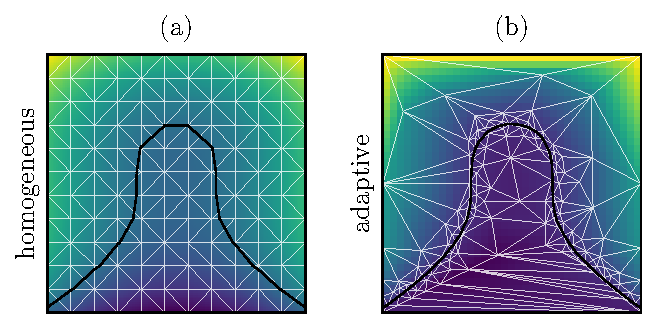
\includegraphics{figures/isoline.pdf}
\caption{Comparison of isoline sampling of \(f(x,y)=x^2 + y^3\) at \(f(x,y)=0.1\) using homogeneous sampling (left) and adaptive sampling (right) with the same amount of points \(n=12^2=144\).
We plot the function interpolated on a grid (color) with the triangulation on top (white) where the function is sampled on the vertices.
The solid line (black) indicates the isoline at \(f(x,y)=0.1\).
The isoline in the homogeneous case consists of 43 line segments and the adaptive case consists of 94 line segments.\label{fig:isoline}}
\end{figure}

\section{Implementation and benchmarks}

\paragraph{The learner abstracts a loss based priority queue.}

We will now introduce Adaptive's API.
The object that can suggest points based on existing data is called a \emph{learner}.
The learner abstracts the sampling strategy based on a priority queue and local loss functions that we described in Sec.~\ref{sec:design}.
We define a learner as follows:

\begin{lstlisting}[language=Python]
from adaptive import Learner1D

def f(x):
    a = 0.01
    return x + a**2 / (a**2 + x**2)

learner = Learner1D(f, bounds=(-1, 1))
\end{lstlisting}

We provide the function to learn, the domain boundaries, and use a default loss function.
We can then \emph{ask} the learner for points:

\begin{lstlisting}[language=Python]
points, priorities = learner.ask(4)
\end{lstlisting}

The learner gives us back the points that we should sample next, as well as the priorities of these points (the loss of the parent subdomains).
We can then evaluate some of these points and \emph{tell} the learner about the results:

\begin{lstlisting}[language=Python]
data = [learner.function(x) for x in points]
learner.tell_many(points, data)
\end{lstlisting}

To change the loss function we pass a function that takes points and values, like so:

\begin{lstlisting}[language=Python]
def distance_loss(xs, ys): # used by default
    dx = xs[1] - xs[0]
    dy = ys[1] - ys[0]
    return np.hypot(dx, dy)

learner = Learner1D(peak, bounds=(-1, 1), loss_per_interval=distance_loss)
\end{lstlisting}

If we wanted to create the ``volume loss'' discussed in Sec.~\ref{sec:loss} we could simply write:

\begin{lstlisting}[language=Python]
def uniform_loss(xs, ys):
    dx = xs[1] - xs[0]
    return dx

learner = Learner1D(peak, bounds=(-1, 1), loss_per_interval=uniform_loss)
\end{lstlisting}

\paragraph{The runner orchestrates the function evaluation.}

The previous example shows how we can drive the learner manually.
For example, to run the learner until the loss is below \passthrough{\lstinline!0.01!} we could do the following:

\begin{lstlisting}[language=Python]
def goal(learner):
    return learner.loss() < 0.01

while not goal(learner):
    (x,), _ = learner.ask(1)
      y = f(x)
      learner.tell(x, y)
\end{lstlisting}

This approach allows for the best \emph{adaptive} performance (i.e.~fewest number of points to reach the goal) because the learner has maximal information about \passthrough{\lstinline!f!} every time we ask it for the next point.
However this does not allow to take advantage of multiple cores, which may enable better \emph{walltime} performance (i.e.~time to reach the goal).
Adaptive abstracts the task of driving the learner and executing \passthrough{\lstinline!f!} in parallel to a \emph{Runner}:

\begin{lstlisting}[language=Python]
from adaptive import Runner
runner = Runner(learner, goal)
\end{lstlisting}

The above code uses the default parallel execution context, which occupies all the cores on the machine.
It is simple to use \emph{ipyparallel} to enable calculations on a cluster:

\begin{lstlisting}[language=Python]
import ipyparallel

runner = Runner(learner, goal, executor=ipyparallel.Client())
\end{lstlisting}

If the above code is run in a Jupyter notebook it will not block.
Adaptive takes advantage of the capabilities of the IPython to execute concurrently with the Python kernel.
This means that as the calculation is in progress the data is accessible without race conditions via \passthrough{\lstinline!learner.data!}, and can be plotted with \passthrough{\lstinline!learner.plot()!}.
Additionally, in a Jupyter notebook environment, we can call \passthrough{\lstinline!runner.live\_info()!} to display useful information about the ongoing calculation.

We have also implemented a \passthrough{\lstinline!LearnerND!} with a similar API

\begin{lstlisting}[language=Python]
from adaptive import LearnerND

def ring(xy): # pretend this is a slow function
    x, y = xy
    a = 0.2
    return x + np.exp(-(x**2 + y**2 - 0.75**2)**2/a**4)

learner = adaptive.LearnerND(ring, bounds=[(-1, 1), (-1, 1)])
runner = Runner(learner, goal)
\end{lstlisting}

Again, it is possible to specify a custom loss function using the \passthrough{\lstinline!loss\_per\_simplex!} argument.

\paragraph{The BalancingLearner can run many learners simultaneously.}

Frequently, more than one function (learner) needs to run at once, to do this we have implemented the \passthrough{\lstinline!BalancingLearner!}, which does not take a function, but a list of learners.
This learner internally asks all child learners for points and will choose the point of the learner that maximizes the loss improvement; it balances the resources over the different learners.
We can use it like

\begin{lstlisting}[language=Python]
from functools import partial
from adaptive import BalancingLearner

def f(x, pow):
    return x**pow

learners = [Learner1D(partial(f, pow=i)), bounds=(-10, 10) for i in range(2, 10)]
bal_learner = BalancingLearner(learners)
runner = Runner(bal_learner, goal)
\end{lstlisting}

For more details on how to use Adaptive, we recommend reading the tutorial inside the documentation \citep{Nijholt2018}.

\section{Possible extensions}

\paragraph{Anisotropic triangulation would improve the algorithm.}

One of the fundamental operations in the adaptive algorithm is selecting a point from within a subdomain.
The current implementation uses simplices for subdomains (triangles in 2D, tetrahedrons in 3D), and picks a point either (1) in the center of the simplex or (2) on the longest edge of the simplex.
The choice depends on the shape of the simplex; the center is only used if using the longest edge would produce unacceptably thin simplices.
A better strategy may be to choose points on the edge of a simplex such that the simplex aligns with the gradient of the function, creating an anisotropic triangulation \citep{Dyn1990}.
This is a similar approach to the anisotropic meshing techniques mentioned in the literature review.

\paragraph{Learning stochastic functions is a promising direction.}

Stochastic processes frequently appear in numerical sciences.
Currently, Adaptive has an \passthrough{\lstinline!AverageLearner!} that samples a random variable (modelled as a function that takes no parameters and returns a different value each time it is called) until the mean is known to within a certain standard error.
This is advantageous because no predetermined number of samples has to be set before starting the simulation.
Extending this learner to be able to deal with stochastic functions in arbitrary dimensions would be a useful addition.

\paragraph{Experimental control needs to deal with noise, hysteresis, and the cost for changing parameters.}

Finally, there is the potential to use Adaptive for experimental control.
There are a number of challenges associated with this use case.
Firstly, experimental results are typically stochastic (due to noise), and would require sampling the same point in parameter space several times.
This aspect is closely associated with sampling stochastic functions discussed in the preceding paragraph.
Secondly, in an experiment one typically cannot jump around arbitrary quickly in parameter space.
It may be faster to sweep one parameter compared to another; for example, in condensed matter physics experiments, sweeping magnetic field is much slower than sweeping voltage source frequency.
Lastly, some experiments exhibit hysteresis.
This means that results may not be reproducible if a different path is taken through parameter space.
In such a case one would need to restrict the sampling to only occur along a certain path in parameter space.
Incorporating such extensions into Adaptive would require adding a significant amount of extra logic, as learners would need to take into account not only the data available, but the order in which the data was obtained, and the timing statistics at different points in parameter space.
Despite these challenges, however, Adaptive can already be used in experiments that are not restricted in these ways.

\section*{Acknowledgements}
We'd like to thank \ldots{}

\section*{Author contributions statement}
Bla


\bibliographystyle{apsrev4-1}
\bibliography{paper.bib}

\end{document}
